\documentclass{article}
\usepackage{amsmath}
\usepackage{algorithm2e}
\usepackage{tabu}
\usepackage{amssymb}
\usepackage{qtree}
\usepackage{comment}
\usepackage{graphicx}
\begin{document}


\title{CS 260: Homework 4}
\author{Daniel Lopez}
\maketitle

\date{22 July 2017}

\section{1}
\subsection{a}
Leaf nodes: D, M, N, F, J, K, L
\subsection{b}
Root node: A
\subsection{c}
Parent node of C: A
\subsection{d}
Node C's children: F, G, H
\subsection{e}
Node ancestors of E: B, A
\subsection{f}
Node descendants of E: I, M, N
\subsection{g}
Right siblings of D and E: none
\subsection{h}
Nodes to the left or right of G: J and K
\subsection{i}
Depth of node C: 1
\subsection{j}
Height of node C:2
\section{2}
1: B E I\newline
2: E I N\newline
3: E I M\newline
4: C H L\newline
5: C G K\newline
6: C G J\newline
\section{3}
\begin{tabu} to 0.8\textwidth { | X[c] | X[c] | X[c] | X[c] | }
	\hline
		& pr(n) $<$ pr(m) & in(n) $<$ in(m) & po(n) $<$ po(m) \\
	\hline
	n is to the left of m & \checkmark & \checkmark & \checkmark  \\
	\hline
	n is to the right of m & \checkmark &  & \checkmark \\
	\hline
	n is a proper ancestor of m & \checkmark & \checkmark &  \\
	\hline
	n is a proper descendant of m &  & \checkmark & \checkmark \\
\hline
\end{tabu}
\section{4}

\Tree[.1 [..45 [.D \textit{.22 00} ]
               [.E \textit{.23 01} ]]
          [..55 [.F \textsc{.27 10} ]
                [..28 [.C \textit{.12 110} ]
                           [..16 [.A \textit{.07 1110} ]
                                [.B \textit{.09 1111} ]]]]]]
\section{5}
\par A tree with n nodes would have a maximum height of n-1 trees to take the root into account. \par
0-1 nodes have a height of 0, 2-3 nodes have a height of 1, 4-7 nodes have a height of 2...so for a binary tree, the minimum height will be $\log_{2} (n)$.\par
\section{6}
With similar logic above, the maximum height will still be n-1 height for n nodes. The minimum height will be $\log_{b} (n)$ for n nodes with b number of children.\linebreak
\linebreak
\begin{comment}
\section{1: Drawing Graphs}
diagraph
{
A [label="6"];
B [label="4"];
C [label="1"];
D [label="10"];
E [label="8"];
null2 [label="null"; shape=none];
null3 [label="null"; shape=none];
A->B;
A->D;
B->C;
B->null2;
D->E;
D->null3;
}
\begin{center}
	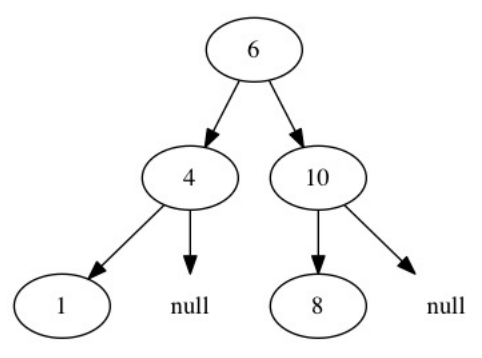
\includegraphics[scale=0.5]{bst_build_05.jpg}
\end{center}
\end{comment}
\end{document}
